% @author Lluis Gesa (lluis.gesa@uab.cat)
%
% Enginyeria Del Software
% -----------------------------------------------------------------------------------



% definim quin estil general volem per el document
\documentclass[11pt]{article}

% indiquem quins paquets amb funcionalitat extra volem fer servir
\usepackage{a4wide, amsmath, tabularx, colortbl, fancyhdr, graphicx, lastpage, caption}
\usepackage[utf8]{inputenc}

% Indiquem que comencem a definir el document i els seus continguts.
\begin{document}

% Definim valors i propietats, creem macros que ens ajudaran a
% agilitzar coses repetides:

\newcommand{\NomProjecte}{Perdidos en la ignorancia}
\newcommand{\NomDocument}{Estado}
\newcommand{\IdentificadorDocument}{GG-SL-N-UC}
\newcommand{\VersioDocument}{v2.0}

% Fent servir propietas del paquet fancyhdr per crear una capçalera
% que es mostrarà cada pàgina
\pagestyle{fancy}
\fancyhead[LO,LE]{
\includegraphics[width = 3.5cm]{./imatges/uab-logo.png}}
\fancyhead[CO,CE]{\bf \NomProjecte \\ \vspace{\baselineskip}
  \NomDocument }
\fancyhead[RO,RE]{
{\bf Ref : \IdentificadorDocument} \\
Versió: \VersioDocument\\
Data: \today \\
Pag. \thepage ~of \pageref{LastPage}
}
\fancyfoot[LO,LE,CO,CE,RO,RE]{}
\textheight=19cm


%
% Creem la pàgina inicial :

% Insertem el nom del document en una taula centrada feng servir una
% font gran \huge

\begin{center}
\begin{tabular*}{15cm}{p{14.5cm}}
\\
\\
\\
\rowcolor[gray]{.9}\begin{center}\huge{\bf{\NomDocument}}\end{center}\\
\\
\end{tabular*}
\end{center}


%
% Insertem una taula que contindrà les abreviacions que hi hagi al
% nostre document
%
\small{%
\begin{center}
\begin{tabular}{|p{2cm}|p{4.75cm}|p{2cm}|p{4.75cm}|}
\hline
\multicolumn{4}{|>{\columncolor[gray]{.9}[2mm][2mm]}c|}{{\bf Abreviatures}} \\
\hline
UAB & Universitat Autonoma de Barcelona & ES & Enginyeria del Software \\
\hline
& & & \\
\hline
\end{tabular}
\end{center}
}

%
% Insertem una taula amb el historial de canvis del document
%
\small{%
\begin{center}
\begin{tabular}{|p{2cm}|p{2cm}|p{7.5cm}|p{2cm}|}
\hline
\multicolumn{4}{|>{\columncolor[gray]{.9}[2mm][2mm]}c|}{{\bf Historial de Revisions}} \\
\hline
{\bf Version} & {\bf Date} & {\bf Comments} & {\bf Autor} \\
\hline
1.0 & 12-Maig-2019 & Sprint 3 &
G43-2-02 \\
\hline
2.0 & 26-Maig-2019 & Sprint 4 &
G43-2-02 \\
\hline
\end{tabular}
\end{center}
}




% Insertem en una nova pàgina, els indexs : de continguts, de figures
% i de taules, les comandes \tableofcontents ,  \listoffigures,
% \listoftables són gestionades per els paquets fets servir, i per
% defecte escriuen els titols de la secció en angles, per canviar-los,
% hem de 'renovar les comandes' :

\renewcommand{\contentsname}{Índex de continguts}
\renewcommand{\listfigurename}{Índex de figures}
\renewcommand{\listtablename}{Índex de taules}

% Ara li diem al LaTeX que inserti la informació
\newpage
\tableofcontents
\listoffigures
\listoftables

% Insertem les seccions que volem
\newpage

\section{Introducció}\label{sec:intro}


En este documento se pretenden recopilar todos los procesos o pruebas necesarias para comprobar que todas las partes del programa funcionan correctamente, es decir, que se ejecutan siguiendo los pasos correctos y responden de la forma esperada. \\ Para ello, se generarán diversos casos de test con la intención de probar todas las posibles combinaciones de entradas/salidas de los múltiples componentes que forman la aplicación.
\section{Estados}\label{sec:uc0}


\subsection{Estado del Juego}\label{sec:uc0}
\begin{center}
  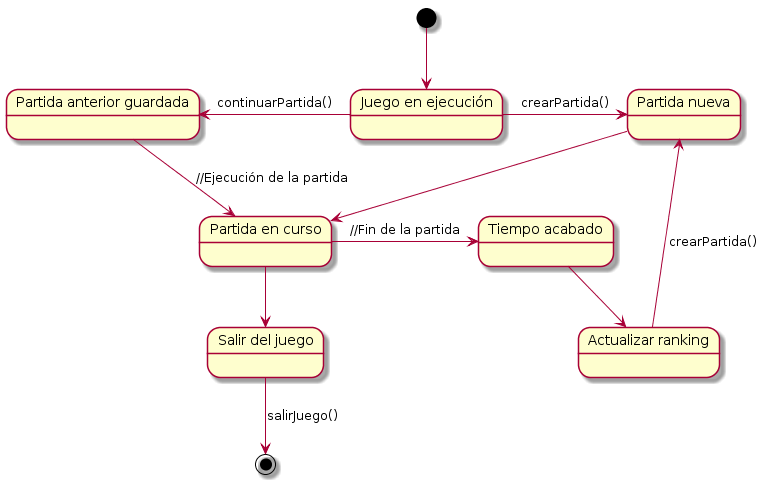
\includegraphics[width=0.9\textwidth]{./imatges/Estados_juego.png}
  \end{center}
  Tenemos que es estado inicial de este diagrama es Juego en ejecución, una vez estamos en este estado tenemos dos opciones, continuar una partida ya existente (partida guardada) o bien, empezar una partida nueva. En ambas situaciones, el proximo estado, es la ejecución de la partida.
  \\A continuación se pueden dar dos casos, uno de ellos es que se haya acabado el tiempo, y por lo tanto la partida finaliza, posteriormente, se pasa a actualizar el ranking, y se empieza una partida nueva.
  \\El segundo caso es que sea el jugador quien desee terminar la partida, en esta situación simplemente se sale del juego, y llegamos al estado final.

% \section{Traçabilitat}\label{sec:intro}

\begin{center}
\begin{tabular}{|c|c|c|}
\hline
{\cellcolor[gray]{.8} \bf Requeriment} & {\cellcolor[gray]{.8} \bf Cas d'ús} & {\cellcolor[gray]{.8} \bf Test}  \\
\hline
REQ-F-1-01 & CU-USUARI-01 & TP-U-01 \\
\hline
REQ-F-1-02 &  & TP-U-01 \\
\hline
REQ-F-1-03 & CU-ADMIN-02 & TP-U-01 \\
\hline
REQ-F-1-04 & CU-ADMIN-03 & TP-U-01 \\
\hline
REQ-F-1-05 & CU-ADMIN-04 & TP-U-01 \\
\hline
REQ-F-1-06 &  & TP-U-01 \\
\hline
REQ-F-1-07 & CU-ADMIN-05 & TP-U-01 \\
\hline
REQ-F-1-08 & CU-ADMIN-06 & TP-U-01 \\
\hline
REQ-F-1-09 &  & TP-U-01 \\
\hline
REQ-F-1-10 & CU-USUARI-07 & TP-U-01 \\
\hline
REQ-F-1-11 & CU-USUARI-08 & TP-U-01 \\
\hline
REQ-F-1-12 & CU-USUARI-09 & TP-U-01 \\
\hline
REQ-F-1-13 & CU-USUARI-10 & TP-U-01 \\
\hline
REQ-F-1-14 & CU-USUARI-11 & TP-U-01 \\
\hline
REQ-F-1-15 & CU-ADMIN-12 & TP-U-01 \\
\hline
REQ-F-1-16 & CU-ADMIN-13 & TP-U-01 \\
\hline
REQ-F-1-17 &  & TP-U-01 \\
\hline
REQ-F-1-18 & CU-USUARI-14 & TP-U-01 \\
\hline
REQ-F-1-19 & CU-USUARI-15 & TP-U-01 \\
\hline
REQ-F-1-20 &  & TP-U-01 \\
\hline
REQ-F-1-21 & CU-SISTEMA-16 & TP-U-01 \\
\hline
REQ-F-1-22 & CU-SISTEMA-17 & TP-U-01 \\
\hline
REQ-F-1-23 & CU-SISTEMA-18 & TP-U-01 \\
\hline
REQ-F-1-24 & CU-SISTEMA-19 & TP-U-01 \\
\hline
REQ-F-1-25 & CU-ADMIN-20 & TP-U-01 \\
\hline
REQ-F-1-26 & CU-USUARI-21 & TP-U-01 \\
\hline
REQ-F-1-27 & CU-USUARI-22 & TP-U-01 \\
\hline
REQ-F-1-28 & CU-USUARI-23 & TP-U-01 \\
\hline
REQ-F-1-29 & CU-USUARI-24 & TP-U-01 \\
\hline
REQ-F-1-30 & CU-USUARI-25 & TP-U-01 \\
\hline
REQ-F-1-31 & CU-ADMIN-26 & TP-U-01 \\
\hline
REQ-F-1-32 & CU-USUARI-27 & TP-U-01 \\
\hline

\end{tabular}
\captionof{table}{Matriu Traçabilitat}
\end{center}


% Finalitzem el document.
\end{document}
